\batchmode

\documentclass[a4paper,english,twoside,openright,11pt]{report}
\RequirePackage{ifthen}




\usepackage[utf8]{inputenc} 
\usepackage{ifpdf}
\usepackage[pdftex]{graphicx}
\usepackage{float}            
\usepackage[english]{babel}   
\usepackage{amstext}          
\usepackage{amsfonts}         
\usepackage{amssymb}          
\usepackage{amsmath}              
\usepackage{bm}               
\usepackage{enumerate}        
\usepackage[bottom]{footmisc} 
\usepackage{array}            
\usepackage{algorithm}        
\usepackage{algorithmic}      
\usepackage{ntheorem}
\usepackage{theorem}
\usepackage{pdfpages}         
\usepackage{parskip}          
\usepackage[right]{eurosym}   
\usepackage{xcolor}           
\usepackage[hyphens]{url}     
\usepackage{makeidx}          
\usepackage{multicol}         
\usepackage{natbib}   
\usepackage[colorlinks,pdfpagelabels,pdfstartview = FitH,bookmarks = true,bookmarksopen = true,bookmarksopen = true,bookmarksnumbered = true,linkcolor = black,plainpages = false,hypertexnames = false,citecolor = black]{hyperref}
\usepackage[colorinlistoftodos, textwidth=4cm, shadow, german]{todonotes}
\usepackage{dlvocab}
\usepackage{xspace}
\usepackage{alltt}
\usepackage{listings}                   
\usepackage{subfig}                             
\usepackage{wrapfig}                    
\usepackage{microtype}


\definecolor{darkred}{rgb}{0.7,0.0,0.0}


\sloppy                       % großzügiger Zeilenumbruch 
                              

%
\renewcommand{\listofalgorithms}% Text "Algoverzeichnis", statt "List of Algos"
{
\begingroup
\listof{algorithm}{Index of algorithms}
\endgroup
}


\lstset{ %
language=Java,                % the language of the code
basicstyle=\footnotesize ,       % the size of the fonts that are used for the code
numbers=left,                   % where to put the line-numbers
numberstyle=\footnotesize ,      % the size of the fonts that are used for the line-numbers
stepnumber=2,                   % the step between two line-numbers. If it's 1, each line 
                                numbersep=5pt,                  % how far the line-numbers are from the code
backgroundcolor=\color{white},  % choose the background color. You must add \usepackage{color}
showspaces=false,               % show spaces adding particular underscores
showstringspaces=false,         % underline spaces within strings
showtabs=false,                 % show tabs within strings adding particular underscores
frame=single,                   % adds a frame around the code
tabsize=2,                      % sets default tabsize to 2 spaces
captionpos=b,                   % sets the caption-position to bottom
breaklines=true,                % sets automatic line breaking
breakatwhitespace=false,        % sets if automatic breaks should only happen at whitespace
title=\lstname,                 % show the filename of files included with \lstinputlisting;
                                escapeinside={\%*}{*)},         % if you want to add a comment within your code
morekeywords={*,...}            % if you want to add more keywords to the set
}


\makeindex % erstelle einen Index bzw. ein Sachverzeichnis)


\theoremstyle{plain}

\newtheorem{theorem}{Theorem}[section] 

\newtheorem{proposition}[theorem]{Proposition} 

\newtheorem{lemma}[theorem]{Lemma} 

\newtheorem{proof}[theorem]{Proof} 

\newtheorem{corollary}[theorem]{Corollary} 

\newtheorem{fact}[theorem]{Fact} 

\newtheorem{axiom}[theorem]{Axiom} 


\newtheorem{odp}{Design Pattern} 


\newtheorem{example}{Example} 

\newtheorem{consider}{Desideratum}[chapter] 


\newtheorem{definition}{Definition}[section] 

\bibliographystyle{ka-style} % Uni-KA-Style

\setlength{\bibsep}{3mm}  % Abstände im Litverzeichnis



\setlength{\unitlength}{1cm} 

\setlength{\oddsidemargin}{0.3cm} 

\setlength{\evensidemargin}{0.3cm} 

\setlength{\textwidth}{15.5cm} 

\setlength{\topmargin}{-1.2cm} 

\setlength{\textheight}{23cm} 
\columnsep 0.5cm



\hyphenation{Samm-lung-en Samm-lung Stau-beck-en Vor-na-me-in-i-ti-al % Ver-st\"ar-ker-aus-gang 
Nach-na-me Kurz-be-zeich-nung deutsch-spra-chige deutsch-sprachig Screen-shot Screen-shots schluss-end-lich Schluss-end-lich Make-In-dex Da-tei-name Da-tei-namen Ur-instinkt Ur-instinkte}  





\pagecolor[gray]{.7}

\usepackage[]{inputenc}



\makeatletter

\makeatletter
\count@=\the\catcode`\_ \catcode`\_=8 
\newenvironment{tex2html_wrap}{}{}%
\catcode`\<=12\catcode`\_=\count@
\newcommand{\providedcommand}[1]{\expandafter\providecommand\csname #1\endcsname}%
\newcommand{\renewedcommand}[1]{\expandafter\providecommand\csname #1\endcsname{}%
  \expandafter\renewcommand\csname #1\endcsname}%
\newcommand{\newedenvironment}[1]{\newenvironment{#1}{}{}\renewenvironment{#1}}%
\let\newedcommand\renewedcommand
\let\renewedenvironment\newedenvironment
\makeatother
\let\mathon=$
\let\mathoff=$
\ifx\AtBeginDocument\undefined \newcommand{\AtBeginDocument}[1]{}\fi
\newbox\sizebox
\setlength{\hoffset}{0pt}\setlength{\voffset}{0pt}
\addtolength{\textheight}{\footskip}\setlength{\footskip}{0pt}
\addtolength{\textheight}{\topmargin}\setlength{\topmargin}{0pt}
\addtolength{\textheight}{\headheight}\setlength{\headheight}{0pt}
\addtolength{\textheight}{\headsep}\setlength{\headsep}{0pt}
\setlength{\textwidth}{349pt}
\newwrite\lthtmlwrite
\makeatletter
\let\realnormalsize=\normalsize
\global\topskip=2sp
\def\preveqno{}\let\real@float=\@float \let\realend@float=\end@float
\def\@float{\let\@savefreelist\@freelist\real@float}
\def\liih@math{\ifmmode$\else\bad@math\fi}
\def\end@float{\realend@float\global\let\@freelist\@savefreelist}
\let\real@dbflt=\@dbflt \let\end@dblfloat=\end@float
\let\@largefloatcheck=\relax
\let\if@boxedmulticols=\iftrue
\def\@dbflt{\let\@savefreelist\@freelist\real@dbflt}
\def\adjustnormalsize{\def\normalsize{\mathsurround=0pt \realnormalsize
 \parindent=0pt\abovedisplayskip=0pt\belowdisplayskip=0pt}%
 \def\phantompar{\csname par\endcsname}\normalsize}%
\def\lthtmltypeout#1{{\let\protect\string \immediate\write\lthtmlwrite{#1}}}%
\newcommand\lthtmlhboxmathA{\adjustnormalsize\setbox\sizebox=\hbox\bgroup\kern.05em }%
\newcommand\lthtmlhboxmathB{\adjustnormalsize\setbox\sizebox=\hbox to\hsize\bgroup\hfill }%
\newcommand\lthtmlvboxmathA{\adjustnormalsize\setbox\sizebox=\vbox\bgroup %
 \let\ifinner=\iffalse \let\)\liih@math }%
\newcommand\lthtmlboxmathZ{\@next\next\@currlist{}{\def\next{\voidb@x}}%
 \expandafter\box\next\egroup}%
\newcommand\lthtmlmathtype[1]{\gdef\lthtmlmathenv{#1}}%
\newcommand\lthtmllogmath{\dimen0\ht\sizebox \advance\dimen0\dp\sizebox
  \ifdim\dimen0>.95\vsize
   \lthtmltypeout{%
*** image for \lthtmlmathenv\space is too tall at \the\dimen0, reducing to .95 vsize ***}%
   \ht\sizebox.95\vsize \dp\sizebox\z@ \fi
  \lthtmltypeout{l2hSize %
:\lthtmlmathenv:\the\ht\sizebox::\the\dp\sizebox::\the\wd\sizebox.\preveqno}}%
\newcommand\lthtmlfigureA[1]{\let\@savefreelist\@freelist
       \lthtmlmathtype{#1}\lthtmlvboxmathA}%
\newcommand\lthtmlpictureA{\bgroup\catcode`\_=8 \lthtmlpictureB}%
\newcommand\lthtmlpictureB[1]{\lthtmlmathtype{#1}\egroup
       \let\@savefreelist\@freelist \lthtmlhboxmathB}%
\newcommand\lthtmlpictureZ[1]{\hfill\lthtmlfigureZ}%
\newcommand\lthtmlfigureZ{\lthtmlboxmathZ\lthtmllogmath\copy\sizebox
       \global\let\@freelist\@savefreelist}%
\newcommand\lthtmldisplayA{\bgroup\catcode`\_=8 \lthtmldisplayAi}%
\newcommand\lthtmldisplayAi[1]{\lthtmlmathtype{#1}\egroup\lthtmlvboxmathA}%
\newcommand\lthtmldisplayB[1]{\edef\preveqno{(\theequation)}%
  \lthtmldisplayA{#1}\let\@eqnnum\relax}%
\newcommand\lthtmldisplayZ{\lthtmlboxmathZ\lthtmllogmath\lthtmlsetmath}%
\newcommand\lthtmlinlinemathA{\bgroup\catcode`\_=8 \lthtmlinlinemathB}
\newcommand\lthtmlinlinemathB[1]{\lthtmlmathtype{#1}\egroup\lthtmlhboxmathA
  \vrule height1.5ex width0pt }%
\newcommand\lthtmlinlineA{\bgroup\catcode`\_=8 \lthtmlinlineB}%
\newcommand\lthtmlinlineB[1]{\lthtmlmathtype{#1}\egroup\lthtmlhboxmathA}%
\newcommand\lthtmlinlineZ{\egroup\expandafter\ifdim\dp\sizebox>0pt %
  \expandafter\centerinlinemath\fi\lthtmllogmath\lthtmlsetinline}
\newcommand\lthtmlinlinemathZ{\egroup\expandafter\ifdim\dp\sizebox>0pt %
  \expandafter\centerinlinemath\fi\lthtmllogmath\lthtmlsetmath}
\newcommand\lthtmlindisplaymathZ{\egroup %
  \centerinlinemath\lthtmllogmath\lthtmlsetmath}
\def\lthtmlsetinline{\hbox{\vrule width.1em \vtop{\vbox{%
  \kern.1em\copy\sizebox}\ifdim\dp\sizebox>0pt\kern.1em\else\kern.3pt\fi
  \ifdim\hsize>\wd\sizebox \hrule depth1pt\fi}}}
\def\lthtmlsetmath{\hbox{\vrule width.1em\kern-.05em\vtop{\vbox{%
  \kern.1em\kern0.8 pt\hbox{\hglue.17em\copy\sizebox\hglue0.8 pt}}\kern.3pt%
  \ifdim\dp\sizebox>0pt\kern.1em\fi \kern0.8 pt%
  \ifdim\hsize>\wd\sizebox \hrule depth1pt\fi}}}
\def\centerinlinemath{%
  \dimen1=\ifdim\ht\sizebox<\dp\sizebox \dp\sizebox\else\ht\sizebox\fi
  \advance\dimen1by.5pt \vrule width0pt height\dimen1 depth\dimen1 
 \dp\sizebox=\dimen1\ht\sizebox=\dimen1\relax}

\def\lthtmlcheckvsize{\ifdim\ht\sizebox<\vsize 
  \ifdim\wd\sizebox<\hsize\expandafter\hfill\fi \expandafter\vfill
  \else\expandafter\vss\fi}%
\providecommand{\selectlanguage}[1]{}%
\makeatletter \tracingstats = 1 
\providecommand{\Beta}{\textrm{B}}
\providecommand{\Mu}{\textrm{M}}
\providecommand{\Kappa}{\textrm{K}}
\providecommand{\Rho}{\textrm{R}}
\providecommand{\Epsilon}{\textrm{E}}
\providecommand{\Chi}{\textrm{X}}
\providecommand{\Iota}{\textrm{J}}
\providecommand{\omicron}{\textrm{o}}
\providecommand{\Zeta}{\textrm{Z}}
\providecommand{\Eta}{\textrm{H}}
\providecommand{\Nu}{\textrm{N}}
\providecommand{\Omicron}{\textrm{O}}
\providecommand{\Tau}{\textrm{T}}
\providecommand{\Alpha}{\textrm{A}}


\begin{document}
\pagestyle{empty}\thispagestyle{empty}\lthtmltypeout{}%
\lthtmltypeout{latex2htmlLength hsize=\the\hsize}\lthtmltypeout{}%
\lthtmltypeout{latex2htmlLength vsize=\the\vsize}\lthtmltypeout{}%
\lthtmltypeout{latex2htmlLength hoffset=\the\hoffset}\lthtmltypeout{}%
\lthtmltypeout{latex2htmlLength voffset=\the\voffset}\lthtmltypeout{}%
\lthtmltypeout{latex2htmlLength topmargin=\the\topmargin}\lthtmltypeout{}%
\lthtmltypeout{latex2htmlLength topskip=\the\topskip}\lthtmltypeout{}%
\lthtmltypeout{latex2htmlLength headheight=\the\headheight}\lthtmltypeout{}%
\lthtmltypeout{latex2htmlLength headsep=\the\headsep}\lthtmltypeout{}%
\lthtmltypeout{latex2htmlLength parskip=\the\parskip}\lthtmltypeout{}%
\lthtmltypeout{latex2htmlLength oddsidemargin=\the\oddsidemargin}\lthtmltypeout{}%
\makeatletter
\if@twoside\lthtmltypeout{latex2htmlLength evensidemargin=\the\evensidemargin}%
\else\lthtmltypeout{latex2htmlLength evensidemargin=\the\oddsidemargin}\fi%
\lthtmltypeout{}%
\makeatother
\setcounter{page}{1}
\onecolumn

% !!! IMAGES START HERE !!!

{\newpage\clearpage
\lthtmlpictureA{tex2html_wrap1622}%

\includegraphics[width=3cm]{BilderAllgemein/KITLogo_RGB.pdf}%
\lthtmlpictureZ
\lthtmlcheckvsize\clearpage}

\stepcounter{chapter}
\stepcounter{section}
\stepcounter{chapter}
\stepcounter{section}
\stepcounter{section}
\stepcounter{subsection}
\stepcounter{subsubsection}
\stepcounter{subsubsection}
\stepcounter{subsection}
{\newpage\clearpage
\lthtmlinlinemathA{tex2html_wrap_inline1675}%
$ N_I$%
\lthtmlinlinemathZ
\lthtmlcheckvsize\clearpage}

{\newpage\clearpage
\lthtmlinlinemathA{tex2html_wrap_inline1677}%
$ N_C$%
\lthtmlinlinemathZ
\lthtmlcheckvsize\clearpage}

{\newpage\clearpage
\lthtmlinlinemathA{tex2html_wrap_inline1679}%
$ N_R$%
\lthtmlinlinemathZ
\lthtmlcheckvsize\clearpage}

{\newpage\clearpage
\lthtmlinlinemathA{tex2html_wrap_inline1681}%
$ \DLConVar{A}\in N_C$%
\lthtmlinlinemathZ
\lthtmlcheckvsize\clearpage}

{\newpage\clearpage
\lthtmlinlinemathA{tex2html_wrap_inline1683}%
$ \top$%
\lthtmlinlinemathZ
\lthtmlcheckvsize\clearpage}

{\newpage\clearpage
\lthtmlinlinemathA{tex2html_wrap_inline1685}%
$ \bot$%
\lthtmlinlinemathZ
\lthtmlcheckvsize\clearpage}

{\newpage\clearpage
\lthtmlinlinemathA{tex2html_wrap_inline1687}%
$ \DLRolVar{R}\in N_R$%
\lthtmlinlinemathZ
\lthtmlcheckvsize\clearpage}

{\newpage\clearpage
\lthtmlinlinemathA{tex2html_wrap_inline1689}%
$ \DLConVar C \DLand \DLConVar D$%
\lthtmlinlinemathZ
\lthtmlcheckvsize\clearpage}

{\newpage\clearpage
\lthtmlinlinemathA{tex2html_wrap_inline1691}%
$ \DLConVar C \DLor \DLConVar D$%
\lthtmlinlinemathZ
\lthtmlcheckvsize\clearpage}

{\newpage\clearpage
\lthtmlinlinemathA{tex2html_wrap_inline1693}%
$ \neg\DLConVar{C}$%
\lthtmlinlinemathZ
\lthtmlcheckvsize\clearpage}

{\newpage\clearpage
\lthtmlinlinemathA{tex2html_wrap_inline1695}%
$ \forall\DLRolVar{R}.\DLConVar C$%
\lthtmlinlinemathZ
\lthtmlcheckvsize\clearpage}

{\newpage\clearpage
\lthtmlinlinemathA{tex2html_wrap_inline1697}%
$ \exists\DLRolVar{R}.\DLConVar C$%
\lthtmlinlinemathZ
\lthtmlcheckvsize\clearpage}

{\newpage\clearpage
\lthtmlinlinemathA{tex2html_wrap_inline1703}%
$ \DLand$%
\lthtmlinlinemathZ
\lthtmlcheckvsize\clearpage}

{\newpage\clearpage
\lthtmlinlinemathA{tex2html_wrap_inline1705}%
$ \DLor$%
\lthtmlinlinemathZ
\lthtmlcheckvsize\clearpage}

{\newpage\clearpage
\lthtmlinlinemathA{tex2html_wrap_inline1707}%
$ \neg C$%
\lthtmlinlinemathZ
\lthtmlcheckvsize\clearpage}

{\newpage\clearpage
\lthtmlinlinemathA{tex2html_wrap_inline1709}%
$ \DLforall{\DLRolVar{R}}{\DLConVar{C}}$%
\lthtmlinlinemathZ
\lthtmlcheckvsize\clearpage}

{\newpage\clearpage
\lthtmlinlinemathA{tex2html_wrap_inline1711}%
$ \DLexists{\DLRolVar{R}}{\DLConVar{ C}}$%
\lthtmlinlinemathZ
\lthtmlcheckvsize\clearpage}

{\newpage\clearpage
\lthtmlinlinemathA{tex2html_wrap_indisplay1713}%
$\displaystyle \DLConVar C, \DLConVar D \rightarrow \DLConVar A \mid \top \mid \bot \mid \DLConVar C \DLand \DLConVar D \mid \DLConVar C \DLor \DLConVar D \mid \neg \DLConVar C \mid \forall \DLRolVar R.\DLConVar C \mid \exists \DLRolVar R.\DLConVar C$%
\lthtmlindisplaymathZ
\lthtmlcheckvsize\clearpage}

{\newpage\clearpage
\lthtmlinlinemathA{tex2html_wrap_inline1715}%
$ \varC\DLsub\varD$%
\lthtmlinlinemathZ
\lthtmlcheckvsize\clearpage}

{\newpage\clearpage
\lthtmlinlinemathA{tex2html_wrap_inline1717}%
$ \varC\DLequiv\varD$%
\lthtmlinlinemathZ
\lthtmlcheckvsize\clearpage}

{\newpage\clearpage
\lthtmlinlinemathA{tex2html_wrap_inline1719}%
$ \varC(\DLIndVar a)$%
\lthtmlinlinemathZ
\lthtmlcheckvsize\clearpage}

{\newpage\clearpage
\lthtmlinlinemathA{tex2html_wrap_inline1721}%
$ \varR(\DLIndVar a, \DLIndVar b)$%
\lthtmlinlinemathZ
\lthtmlcheckvsize\clearpage}

{\newpage\clearpage
\lthtmlinlinemathA{tex2html_wrap_inline1723}%
$ \Sigma({\cal O})$%
\lthtmlinlinemathZ
\lthtmlcheckvsize\clearpage}

{\newpage\clearpage
\lthtmlinlinemathA{tex2html_wrap_inline1727}%
$ \DLConVar{Pizza},\DLConVar{CheeseTopping} \in N_C, \DLRolVar{hasTopping} \in N_R$%
\lthtmlinlinemathZ
\lthtmlcheckvsize\clearpage}

{\newpage\clearpage
\lthtmlinlinemathA{tex2html_wrap_indisplay1729}%
$\displaystyle (\DLConVar{Pizza} \DLand \forall \DLRolVar{hasTopping}.\DLConVar{CheeseTopping}) \sqsubseteq \DLConVar{CheeseyPizza}$%
\lthtmlindisplaymathZ
\lthtmlcheckvsize\clearpage}

\stepcounter{subsection}
\stepcounter{subsubsection}
\stepcounter{subsection}
\stepcounter{subsubsection}
\stepcounter{subsubsection}
\stepcounter{subsubsection}
\stepcounter{section}
\stepcounter{subsection}
\stepcounter{subsubsection}
\stepcounter{subsubsection}
\stepcounter{subsection}
\stepcounter{section}
\stepcounter{subsection}
\stepcounter{subsection}
\stepcounter{chapter}
\stepcounter{section}
\stepcounter{subsection}
\stepcounter{subsection}
\stepcounter{subsection}
\stepcounter{section}
\stepcounter{subsection}
{\newpage\clearpage
\lthtmlpictureA{tex2html_wrap1086}%
\rotatebox{0}{
                                        \resizebox{!}{0.6\textwidth}{
                                                \fbox{
                                                        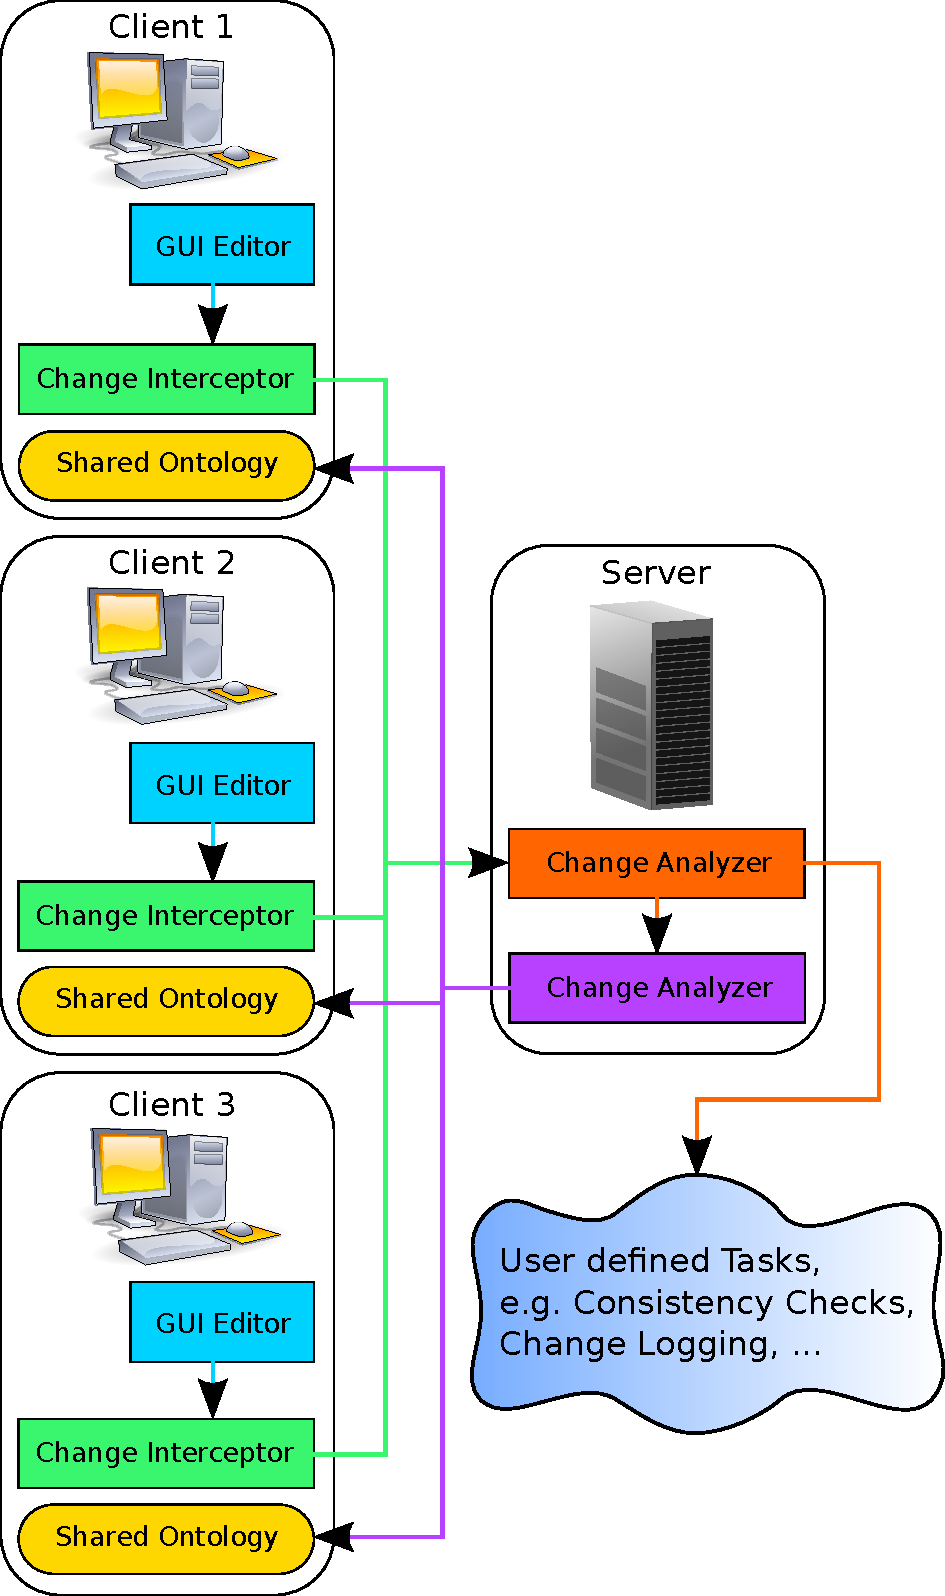
\includegraphics{BilderFrameworkArch/scenario0.pdf}
                                                }
                                        }
                                }%
\lthtmlpictureZ
\lthtmlcheckvsize\clearpage}

{\newpage\clearpage
\lthtmlpictureA{tex2html_wrap1088}%
\rotatebox{0}{
                                        \resizebox{!}{0.6\textwidth}{
                                                \fbox{
                                                        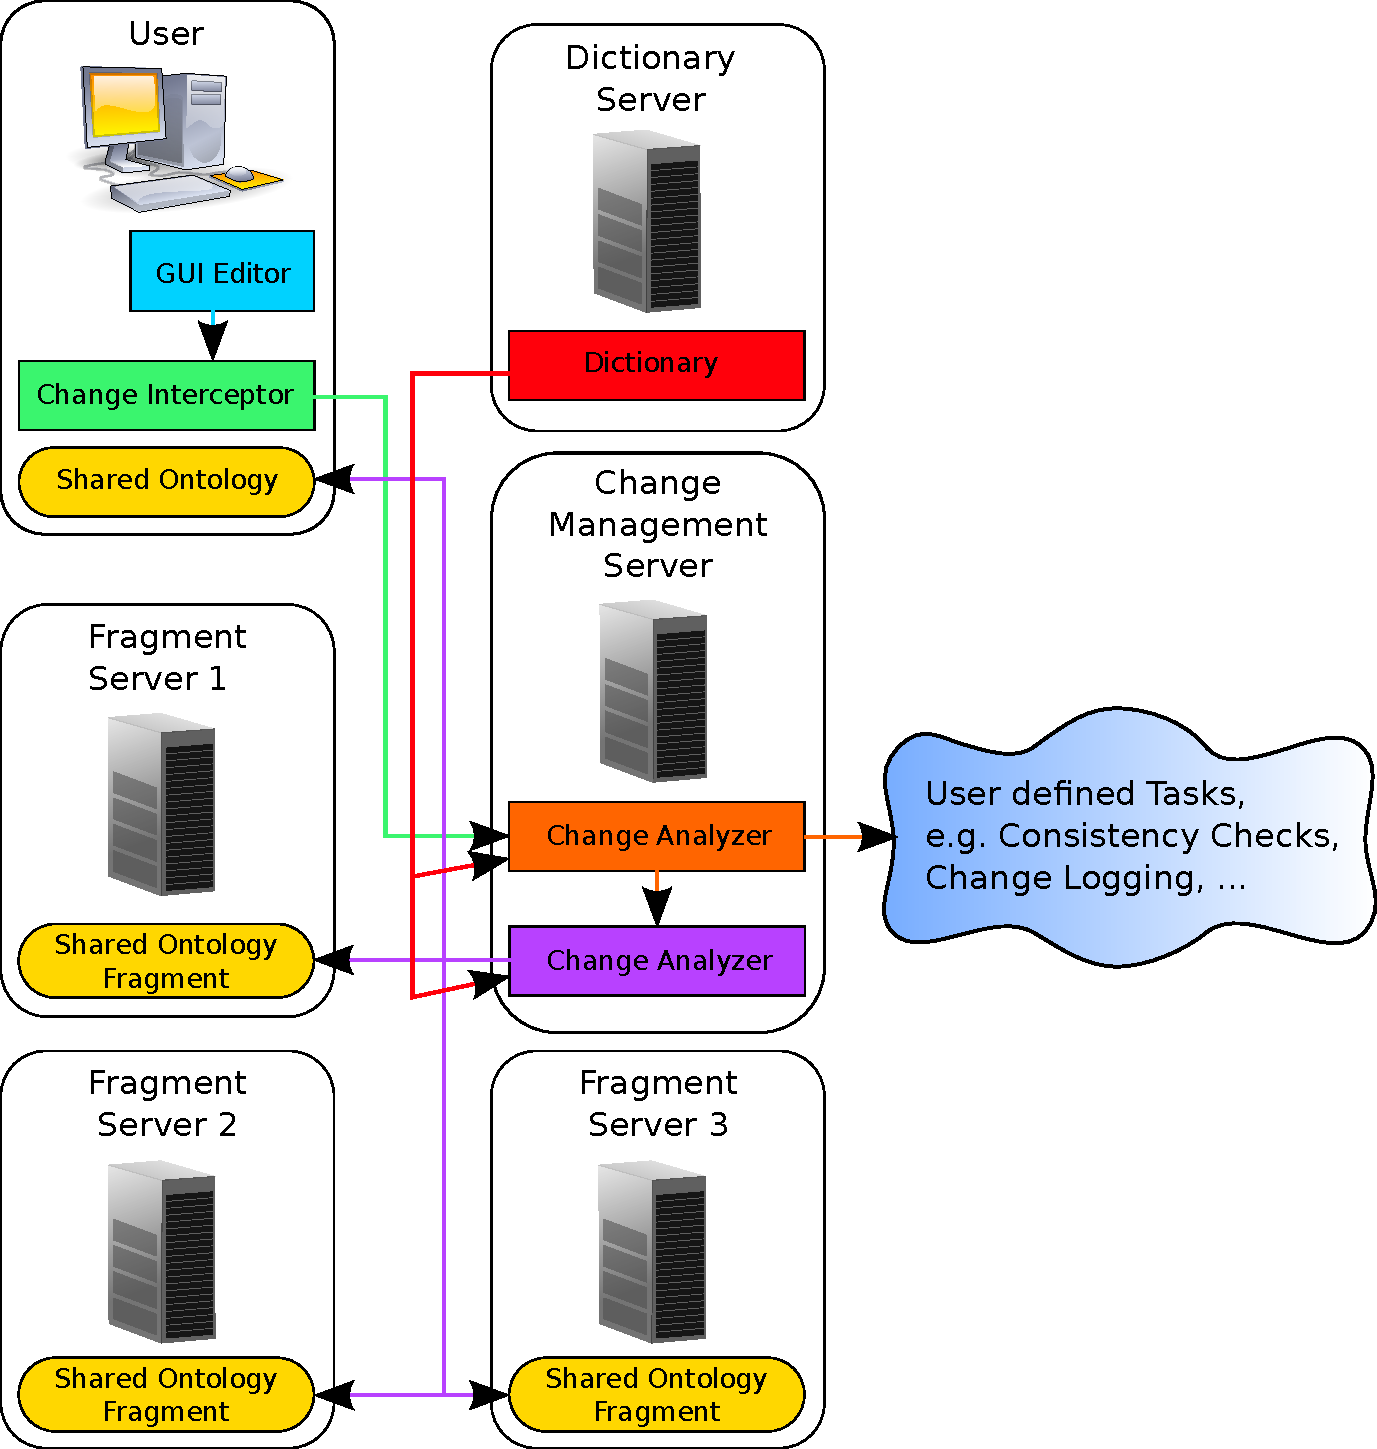
\includegraphics{BilderFrameworkArch/scenario1.pdf}
                                                }
                                        }
                                }%
\lthtmlpictureZ
\lthtmlcheckvsize\clearpage}

\stepcounter{subsection}
{\newpage\clearpage
\lthtmlinlinemathA{tex2html_wrap_inline1823}%
$ o$%
\lthtmlinlinemathZ
\lthtmlcheckvsize\clearpage}

{\newpage\clearpage
\lthtmlinlinemathA{tex2html_wrap_inline1825}%
$ \varphi$%
\lthtmlinlinemathZ
\lthtmlcheckvsize\clearpage}

{\newpage\clearpage
\lthtmlinlinemathA{tex2html_wrap_inline1829}%
$ \varphi\subseteq o$%
\lthtmlinlinemathZ
\lthtmlcheckvsize\clearpage}

\stepcounter{subsection}
{\newpage\clearpage
\lthtmlinlinemathA{tex2html_wrap_inline1837}%
$ \mathcal{I}$%
\lthtmlinlinemathZ
\lthtmlcheckvsize\clearpage}

{\newpage\clearpage
\lthtmlinlinemathA{tex2html_wrap_inline1839}%
$ \mathcal{F}$%
\lthtmlinlinemathZ
\lthtmlcheckvsize\clearpage}

{\newpage\clearpage
\lthtmlinlinemathA{tex2html_wrap_inline1841}%
$ \phi$%
\lthtmlinlinemathZ
\lthtmlcheckvsize\clearpage}

{\newpage\clearpage
\lthtmlinlinemathA{tex2html_wrap_inline1843}%
$ \mathcal{I} \to \mathcal{F}$%
\lthtmlinlinemathZ
\lthtmlcheckvsize\clearpage}

{\newpage\clearpage
\lthtmlinlinemathA{tex2html_wrap_inline1854}%
$ \varphi \in \mathcal{F}$%
\lthtmlinlinemathZ
\lthtmlcheckvsize\clearpage}

{\newpage\clearpage
\lthtmlinlinemathA{tex2html_wrap_inline1856}%
$ \iota$%
\lthtmlinlinemathZ
\lthtmlcheckvsize\clearpage}

{\newpage\clearpage
\lthtmlinlinemathA{tex2html_wrap_inline1862}%
$ \exists \iota \in \mathcal{I} : \phi(\iota) = \varphi$%
\lthtmlinlinemathZ
\lthtmlcheckvsize\clearpage}

{\newpage\clearpage
\lthtmlinlinemathA{tex2html_wrap_inline1869}%
$ \mathcal{I}_\varphi$%
\lthtmlinlinemathZ
\lthtmlcheckvsize\clearpage}

{\newpage\clearpage
\lthtmlinlinemathA{tex2html_wrap_inline1873}%
$ \Sigma = \{{\sigma(\varphi)}\mid\varphi\in{\cal F}\}
$%
\lthtmlinlinemathZ
\lthtmlcheckvsize\clearpage}

{\newpage\clearpage
\lthtmlinlinemathA{tex2html_wrap_inline1877}%
$ {\cal I}_\varphi$%
\lthtmlinlinemathZ
\lthtmlcheckvsize\clearpage}

{\newpage\clearpage
\lthtmlinlinemathA{tex2html_wrap_inline1879}%
$ \cal F$%
\lthtmlinlinemathZ
\lthtmlcheckvsize\clearpage}

{\newpage\clearpage
\lthtmlinlinemathA{tex2html_wrap_inline1881}%
$ \mathcal{D} = \{\mathcal{I}_\varphi, \Sigma, \phi \}$%
\lthtmlinlinemathZ
\lthtmlcheckvsize\clearpage}

\stepcounter{subsection}
{\newpage\clearpage
\lthtmlinlinemathA{tex2html_wrap_inline1895}%
$ \mathcal{D}$%
\lthtmlinlinemathZ
\lthtmlcheckvsize\clearpage}

{\newpage\clearpage
\lthtmlinlinemathA{tex2html_wrap_inline1897}%
$ \{o,\mathcal{F},\mathcal{D}\}$%
\lthtmlinlinemathZ
\lthtmlcheckvsize\clearpage}

\stepcounter{subsection}
\stepcounter{subsubsection}
{\newpage\clearpage
\lthtmlinlinemathA{tex2html_wrap_inline1906}%
$ \Delta$%
\lthtmlinlinemathZ
\lthtmlcheckvsize\clearpage}

{\newpage\clearpage
\lthtmlinlinemathA{tex2html_wrap_inline1908}%
$ \upsilon$%
\lthtmlinlinemathZ
\lthtmlcheckvsize\clearpage}

{\newpage\clearpage
\lthtmlinlinemathA{tex2html_wrap_inline1910}%
$ \tau$%
\lthtmlinlinemathZ
\lthtmlcheckvsize\clearpage}

{\newpage\clearpage
\lthtmlinlinemathA{tex2html_wrap_inline1912}%
$ \omega$%
\lthtmlinlinemathZ
\lthtmlcheckvsize\clearpage}

{\newpage\clearpage
\lthtmlinlinemathA{tex2html_wrap_inline1914}%
$ \mathcal{\nu} = \{\Delta, \upsilon, \tau, \omega \}$%
\lthtmlinlinemathZ
\lthtmlcheckvsize\clearpage}

{\newpage\clearpage
\lthtmlinlinemathA{tex2html_wrap_inline1921}%
$ Change \to Boolean$%
\lthtmlinlinemathZ
\lthtmlcheckvsize\clearpage}

{\newpage\clearpage
\lthtmlinlinemathA{tex2html_wrap_inline1928}%
$ n \in \mathbb{N}$%
\lthtmlinlinemathZ
\lthtmlcheckvsize\clearpage}

{\newpage\clearpage
\lthtmlinlinemathA{tex2html_wrap_inline1930}%
$ \gamma_i$%
\lthtmlinlinemathZ
\lthtmlcheckvsize\clearpage}

{\newpage\clearpage
\lthtmlinlinemathA{tex2html_wrap_inline1932}%
$ \Theta = \bigcup_{i=0..n} \gamma_i$%
\lthtmlinlinemathZ
\lthtmlcheckvsize\clearpage}

\stepcounter{subsubsection}
{\newpage\clearpage
\lthtmlpictureA{tex2html_wrap1134}%
\rotatebox{-90}{
                        \resizebox{!}{10cm}{
                                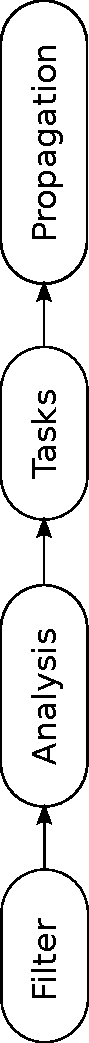
\includegraphics[width=10cm]{BilderFrameworkArch/change_processing_flow.pdf}
                        }
                }%
\lthtmlpictureZ
\lthtmlcheckvsize\clearpage}

{\newpage\clearpage
\lthtmlfigureA{algorithm866}%
\begin{algorithm}
% latex2html id marker 866
[h]                      % enter the algorithm environment
\caption{\textsc{ApplyChange($\mathcal{\nu}$)}}          % give the algorithm a caption
% and a label for \ref{} commands later in the document
\begin{algorithmic}[h]                    % enter the algorithmic environment
\REQUIRE Shared Ontology $o$, Change Filter $\Theta$
\IF{\NOT \textsc{Filter($\mathcal{\nu}, \Theta$)}}
        \STATE{$\alpha \leftarrow \textsc{Analyse($\mathcal{\nu}$)}$
        \STATE \textsc{Trigger($\alpha$)}
        \STATE \textsc{Propagate($\alpha,\mathcal{\nu}$)}}
        \RETURN applied changes on $o$
\ELSE
        \STATE // ignore change
\ENDIF
\end{algorithmic}
\end{algorithm}%
\lthtmlfigureZ
\lthtmlcheckvsize\clearpage}

{\newpage\clearpage
\lthtmlfigureA{algorithm877}%
\begin{algorithm}
% latex2html id marker 877
[h]                      % enter the algorithm environment
\caption{\textsc{Filter($\mathcal{\nu}, \Theta$)}}          % give the algorithm a caption
% and a label for \ref{} commands later in the document
\begin{algorithmic}[h]                    % enter the algorithmic environment
\REQUIRE Criteria $\chi_i \in \Theta$\hspace{0,5cm} $i = 1,2,...,n$\hspace{0,5cm} $i,n \in \mathbb{N}$
\FOR{$i = 1\text{ to }n$}
        \IF{$\chi_i(\mathcal{\nu})$}
                \RETURN \TRUE
        \ENDIF
\ENDFOR
\RETURN \FALSE
\end{algorithmic}
\end{algorithm}%
\lthtmlfigureZ
\lthtmlcheckvsize\clearpage}

\stepcounter{subsubsection}
\stepcounter{subsubsection}
\stepcounter{subsubsection}
\stepcounter{subsection}
\stepcounter{section}
\stepcounter{subsection}
\stepcounter{subsubsection}
\stepcounter{section}
\stepcounter{chapter}
\stepcounter{section}
\stepcounter{subsection}
\stepcounter{subsection}
\stepcounter{section}
\stepcounter{subsection}
\stepcounter{subsection}
\stepcounter{subsection}
\stepcounter{section}
\stepcounter{subsection}
\stepcounter{section}
\stepcounter{subsection}
\stepcounter{subsubsection}
\stepcounter{subsection}
\stepcounter{section}
\stepcounter{section}
\stepcounter{subsection}
\stepcounter{subsection}
\stepcounter{subsection}
\stepcounter{subsection}
\stepcounter{chapter}
\stepcounter{section}
\stepcounter{subsection}
\stepcounter{subsection}
\stepcounter{section}
\stepcounter{chapter}
\stepcounter{chapter}
{\newpage\clearpage
\lthtmlfigureA{lstlisting1561}%
\begin{lstlisting}[caption={The \emph{applyChanges} method of
	the OWLReplicaOntology implementation},label=applyChange]
@ProxyMethod
@PropagatingMethod
public List<OWLOntologyChange> applyChange(OWLOntologyChange change) {
		final SharedObjectMsg msg = SharedObjectMsg.createMsg("applyChangeSilent", change);
		try {
			// Send change to everyone
			sendSharedObjectMsgTo(null, msg);
		} catch (IOException e) {
			// Error processing
			e.printStackTrace();
		}
		if(calledByOntologyManager()) {
			return ontology.applyChange(change);
		}
		return ontology.getOWLOntologyManager().applyChange(change);
	}
\end{lstlisting}%
\lthtmlfigureZ
\lthtmlcheckvsize\clearpage}

{\newpage\clearpage
\lthtmlfigureA{lstlisting1567}%
\begin{lstlisting}[caption={The \emph{applyChangesSilent} method of
	the OWLReplicaOntology implementation},label=applyChangesSilent]
		public void applyChangeSilent(OWLOntologyChange change) {
	change.setOntology(ontology);
	ontology.getOWLOntologyManager().applyChange(change);
}
\end{lstlisting}%
\lthtmlfigureZ
\lthtmlcheckvsize\clearpage}

{\newpage\clearpage
\lthtmlfigureA{lstlisting1571}%
\begin{lstlisting}
% latex2html id marker 1571
[caption={Example of OWL axioms},label=owlclass,language=XML]
	<owl:Class rdf:about="#CheeseTopping">
		<rdfs:label xml:lang="pt">CoberturaDeQueijo</rdfs:label>
		<rdfs:subClassOf>
			<owl:Class rdf:about="#PizzaTopping"/>
		</rdfs:subClassOf>
	</owl:Class>
\end{lstlisting}%
\lthtmlfigureZ
\lthtmlcheckvsize\clearpage}


\end{document}
